%\documentclass[11pt, twocolumn]{article}
\documentclass[11pt]{article}
\usepackage{multicol}
\usepackage{pslatex}
\usepackage{amsmath}
\usepackage{amssymb}
\usepackage{amsthm}
\usepackage{graphicx}
\usepackage{mathrsfs}
\usepackage{algorithmic}
\usepackage{algorithm}
\usepackage{subfig}
\usepackage{url}
%\usepackage[left=.75in,top=.75in,right=.75in,bottom=.75in]{geometry}
\usepackage[left=1in,top=1.2in,right=1in,bottom=1in]{geometry}

\textwidth 6.5in
\textheight 8.8in

\title{TrackMeNot-so-good-after-all}
\author{Rami Al-Rfou' \\{\texttt{ralrfou@cs.stonybrook.edu}}
\and William Jannen \\{\texttt{wjannen@cs.stonybrook.edu}}
\and Nikhil Patwardhan \\{\texttt{npatwardhan@cs.stonybrook.edu}}
}
\begin{document}

\maketitle

\pagestyle{headings}

\begin{abstract}
  TrackMeNot is a Firefox plugin with laudable intentions - protecting
  your privacy. By issuing a customizable stream of random search
  queries on its users' behalf, it surmises that enough ``search
  noise'' will prevent the users' true query profiles from being
  discerned. However, we find that clustering queries by semantic
  relatedness allows us to disentangle a nontrivial subset of user
  queries from TrackMeNot issued noise.
\end{abstract}
\begin{multicols}{2}
\section{Background}
\label{sec:background}
%Identity theft is a major issue in moern society; as many as 10
%million Americans are victims of identity theft each year
%\cite{spamlaws}. As awareness spreads, the issue of online privacy has
%come into focus as a way to reduce exposure.  

The decreasing cost of persistant media for storage, coupled with the
steady rise in E-commerce, social networking, and various other online
services, has led to a dramatic increase in the volume of readily
available, personally identifiable information. One often overlooked
source of such information is the logging by search engines of user
queries.

There have been several high-profile examples of this type of data
being used in inappropriate ways, most notably an incident involving AOL in 2006 \cite{aol}. The company disclosed a data set comprised of  information from 658,000
subscribers' search terms; it was released as a flat file into the public
domain. Upon admitting their error, they removed the link, but the data was already mirrored elsewhere. This incident highlights just how personally revealing search
engine queries can be, as at least one user was identified using only
the content of her searches \cite{user957}.

The average internet user may browse under the false impression that
deleting cookies or diverting traffic through a proxy will protect
their anonymity on the web. Neither of these measures provide complete
protection. If a user wishes to utilize certain services such as
Google Mail, they must log in to their personal profile. Once logged
in, their queries are then tied to their accout.

TrackMeNot is a Firefox plugin that aims to protect the privacy of its users by issuing random queries on their behalf. These random queries are pulled from a variety of sources, with the intuition that providing enough ``noise'' around a user's true search patterns will make it impossible to disentangle the queries made by TrackMeNot from those actually made by human searchers.

\section{TrackMeNot details}
\label{sec:tmn}
TrackMeNot operates completely on the client side as a Firefox plugin. Upon startup, an initial {\it seed list} is populated from RSS feeds and known public ``popular search'' lists. During execution, queries are pulled from this list and issued to popular search engines on the user's behalf.

TrackMeNot takes several steps in an attempt to simulate real user behavior. The basis of the model is its {\it dynamic query list}. Starting from the initial seed list, queries are randomly marked for replacement over time. When a marked query is sent to as a search engine request, the HTTP responses are parsed using a regular expressions to find potential ``query-like'' terms. If a suitable term is found, it is then substituted for the marked query. In this way, the list of searches will evolve over time.

TrackMeNot also attempts to simulate search patterns with ``selective click-through''. 

\section{Design}
\label{sec:design}
Our overall design can be logically divided into three parts. The first part deals with logging all user Google Search queries as well as those fired from TMN. The second part comprises the computation of a distance matrix on this set of queries using a suitable semantic distance measure. The last part consists of clustering this data using a suitable technique to get a visual representation of the data from which conclusions can be deduced.

\subsection{Data Gathering}

\subsection{Semantic Distance Metric}
The basic idea here was to find how \textit{similar} each search query was to every other query, making no distinction based on its origin (user or TMN). To do this, we needed a \textit{semantic} distance metric. We did not implement our own metric, but instead explored the available choices from other research groups. After examining the feasibility of using different available metrics, we settled on two of them. One of them is DISCO\footnote{http://www.linguatools.de/disco/disco\_en.html}, which is a Java package, and the other is Google Normalized Distance. We describe both in the following sections. In each of these cases, we disabled the auto-complete feature of Google so that our search queries were always the exact phrases that the user or TMN requested from Google Search and never subsets of the actual queries.

\subsubsection{DISCO}
The DISCO (extracting DIStributionally related words using CO-occurrences) API allows to compute the semantic similarity between any two words by looking up those words in a pre-defined repository. For our analysis, we downloaded the Wikipedia repository available on the DISCO website to compute the distances. By looking up this local repository, the DISCO API returns a value between 0 and 1 for any pair of words that it looks up in the repository, such that the higher the value returned, the more similar the words are. In this sense, the API works like a similarity measure. We were however faced with one issue: Google search queries are typically phrases, and not single words. To overcome this, given two queries $Q1$ and $Q2$, we compared each word in $Q1$ with every word in $Q2$ and in each case chose the highest retured value. We aggregated this score over all words in $Q1$ and normalized the addition by dividing the aggregate score by the number of words in $Q1$.

\subsubsection{Google Normalized Distance}

\subsection{Clustering}
\label{sec:clustering}
PAM.

\section{Results}
\label{sec:results}

Results. \cite{tmn}

  \begin{figure}[h]
    \centering
    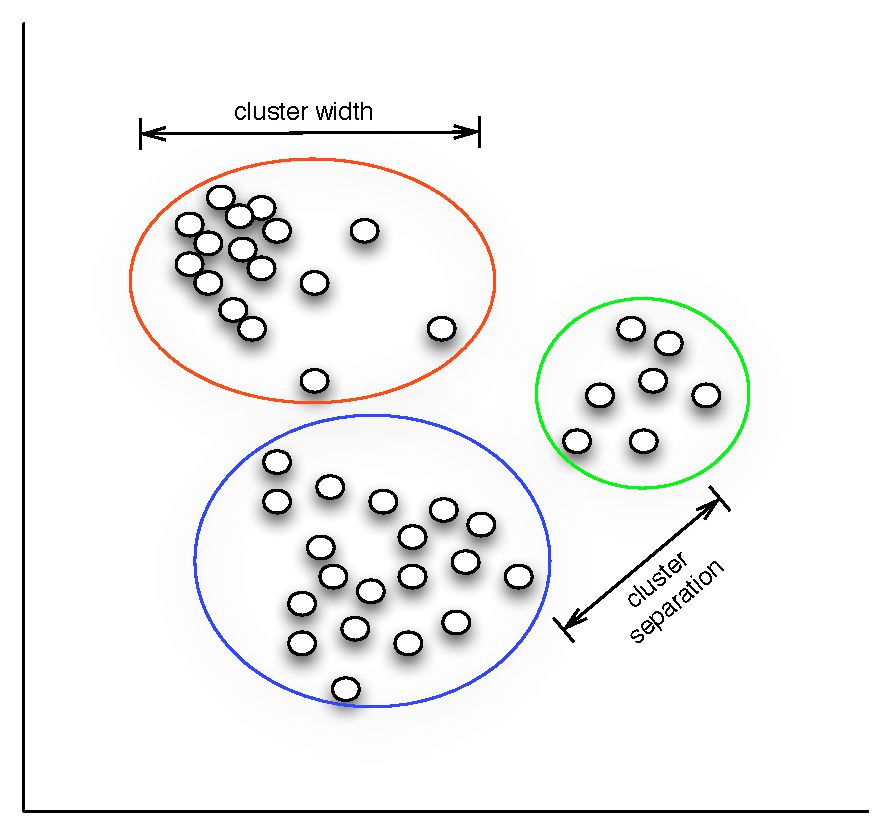
\includegraphics[width=\columnwidth]{clusterbill1}
    \caption{Clustering of bills data.}
    \label{fig:cluster.bill}
  \end{figure}

\section{Conclusions}
\label{sec:conc}
Conclusions.

\section{Future work}
\label{sec:future}
By operating as a Firefox plugin, TrackMeNot does not protect against search engines tracking time of use. As a standalone application, TrackMeNot could be run in the background, even while a user is not actively browsing. This would not only provide the same semantic search noise as the current TrackMeNot implementation, but it would serve to protect the temporal search habits of users.



\bibliographystyle{abbrv}
\bibliography{final_report}
\end{multicols}
\newpage
\begin{appendix} \label{appendix}
\section*{Appendix:}
{\tiny
\begin{verbatim}
Appendix info.
\end{verbatim}
}
\end{appendix}

\end{document}